\section{System Overview \& Main Techniques}
\label{sec:approach}

\begin{figure}[t]
\centering
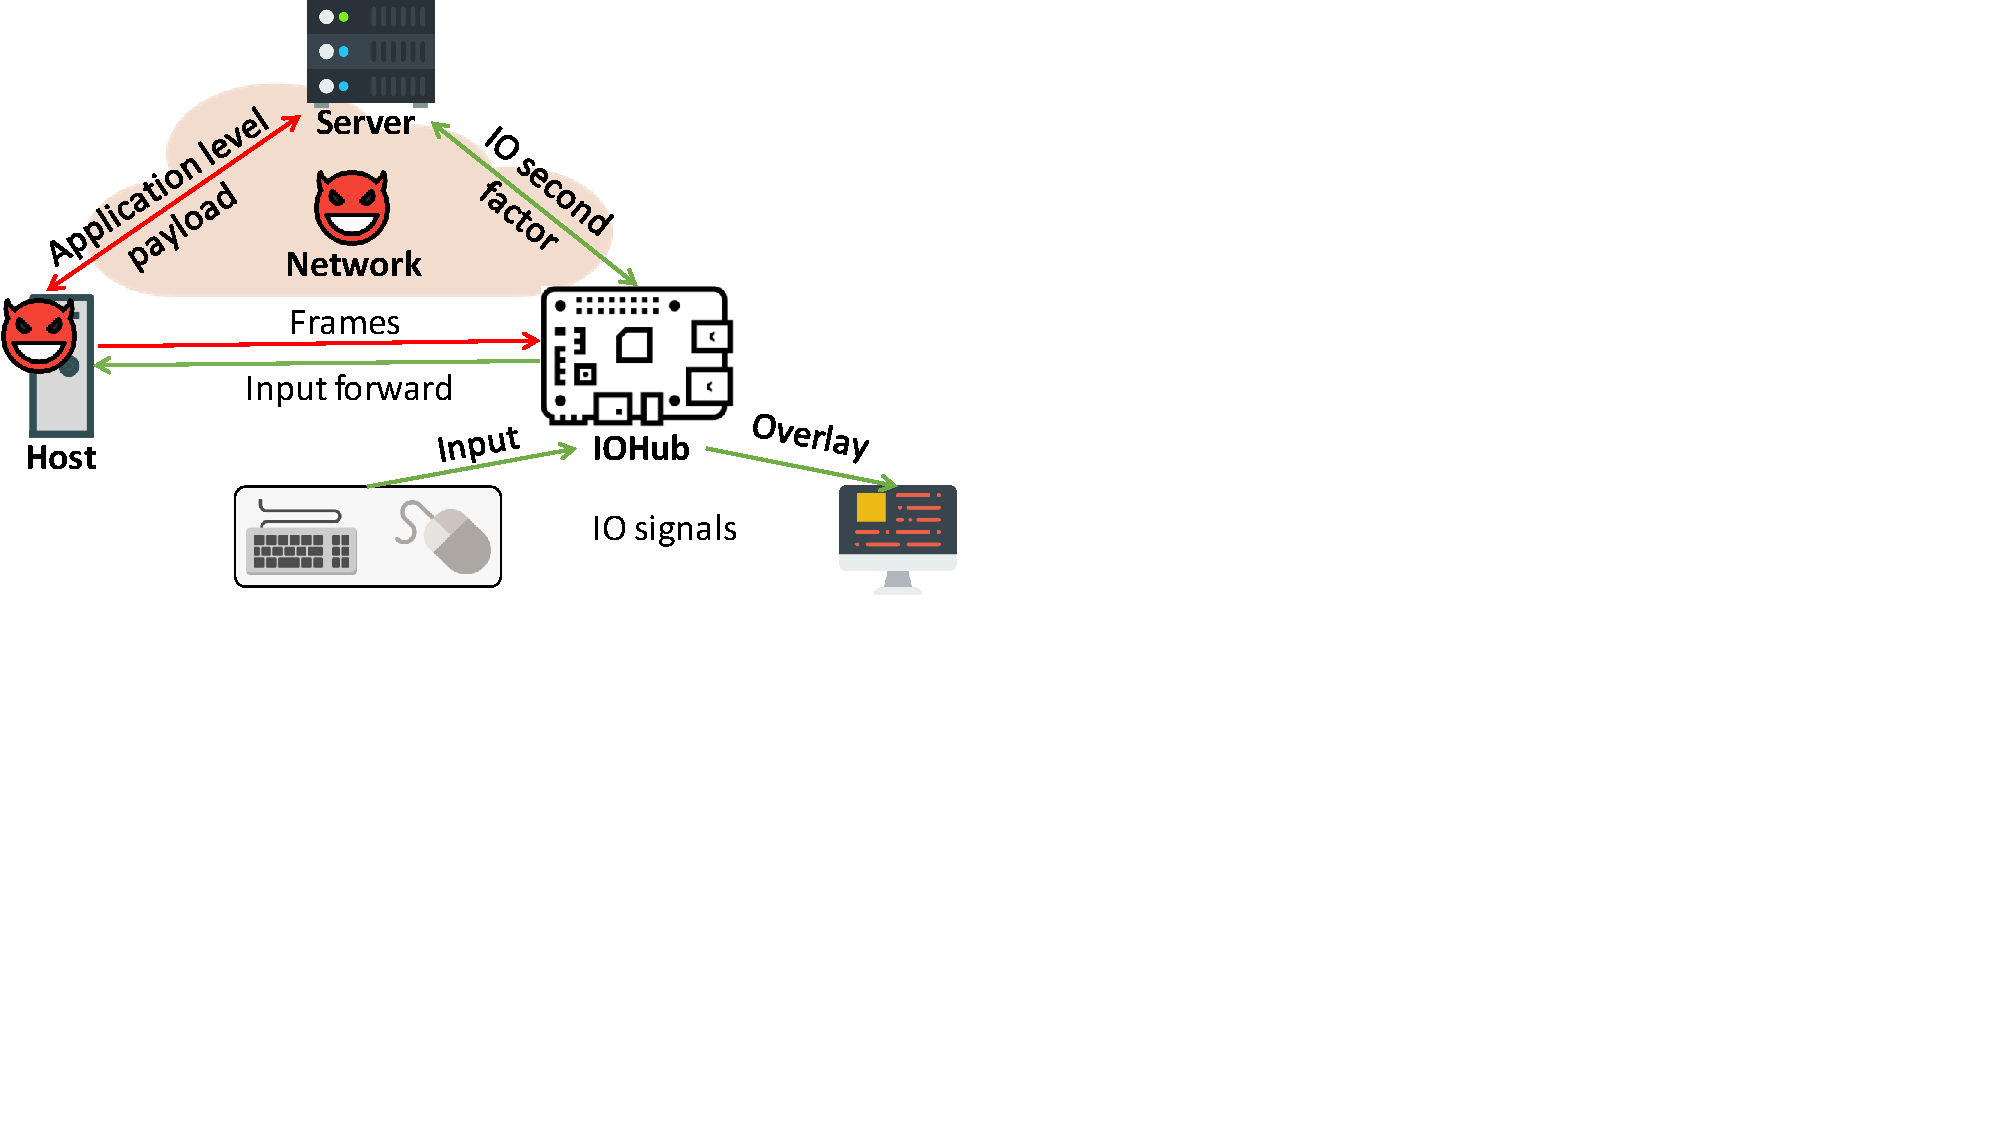
\includegraphics[trim={0 8.5cm 17cm 0}, clip, width=0.85\linewidth]{chapters/ProtectIOn/images/approachOverview.pdf}
\caption[High-level approach overview of \name]{\textbf{High-level approach overview of our solution.}  The \device connects the trusted IO devices and the attacker-controlled host.}
\label{fig:approachOverview}
\centering
\end{figure}



In this section, we present an overview of our solution: \name. On the high-level, \name uses the concept of the \emph{bump in the wire} (such as bump in the ether~\cite{McCPerRei2006}) to provide integrity and confidentiality to the user IO{}s between the IO devices and the remote server. \name achieves this by utilizing a trusted embedded device as a mediator between all the IO devices and the untrusted host. Hence, our approach falls into the category \textbf{B2} (external HW) in Figure~\ref{fig:relatedWorksTree}. We call this trusted intermediary \device. 


\subsection{System and Attacker Model}
\label{sec:approach:systemAttackerModel}

We consider a typical scenario where the user wants to interact with a trusted remote web server via an attacker-controlled host. The model is depicted in Figure~\ref{fig:approachOverview}, which shows the untrusted host, the remote server, and the user IO devices. We only assume that the monitor, keyboard, mouse (in a word all the IO devices that we need to protect from the malicious host), and the \device are trusted. One benefit of an external trusted device is that regulations may prevent modifications of systems such as medical devices. However, retrofitting them with external devices, such as the IOHub, is usually possible.

The \device works as a mediator between all the IO devices and the host. Note that the \device has no network capability to communicate with the server directly, instead it relies on the host and uses it as an untrusted transport. We also assume that the \device comes with preloaded certificates and keys that allow the \device to verify the signatures signed by the server and sign data such as the user input.

\myparagraph{Deployment options}
There are several possible ways to deploy the \name system. Here we outline two example cases. The first example deployment is one where a service provider, like a bank issues a \device device to each of its customers. In such a deployment, the issued \device is intended to be used with a single application like a web-based online banking application, and it is pre-configured with the public key certificate of that application server (e.g., online banking server). The pre-installed certificate allows the \device to verify messages signed by the correct application server. The service provider (i.e., the issuer of the \device) can ask what OS the customer uses and configure OS-specific settings like the used SAS value to the issued device (see Section~\ref{sec:confidentiality:SAS} for details). 
%Another option is that the \device is issued by a service provider who also runs the remote server. \red{(\#2)Based on the specific application, \device could be adapted. E.g., safety-critical system administrator may opt to use a \device that is specific for a given application. Financial institutions may also follow the similar approach. 

In another example deployment, the \device is issued by a third-party vendor, and it is intended to be used to protect the user interaction of various security-critical online services. In such a deployment, the \device can be pre-configured with the public key of its issuer and a white-list of trusted application server certificates. The issuer of the device can issue authenticated updates to the white-list after its deployment if needed.

\myparagraph{Attacker model and capabilities} Our attacker model assumes that the host (OS, installed applications, and hardware) and the network are attacker-controlled. The attacker can intercept, and arbitrarily manipulate (such as create, drop, or modify) the user IO data between the user and the remote server. Furthermore, we assume that the attacker can not break the physical security of the \device (more discussion in Section~\ref{sec:securityAnalysis:device}).



\subsection{High-level Description of the System}

\begin{figure}[t]
\centering
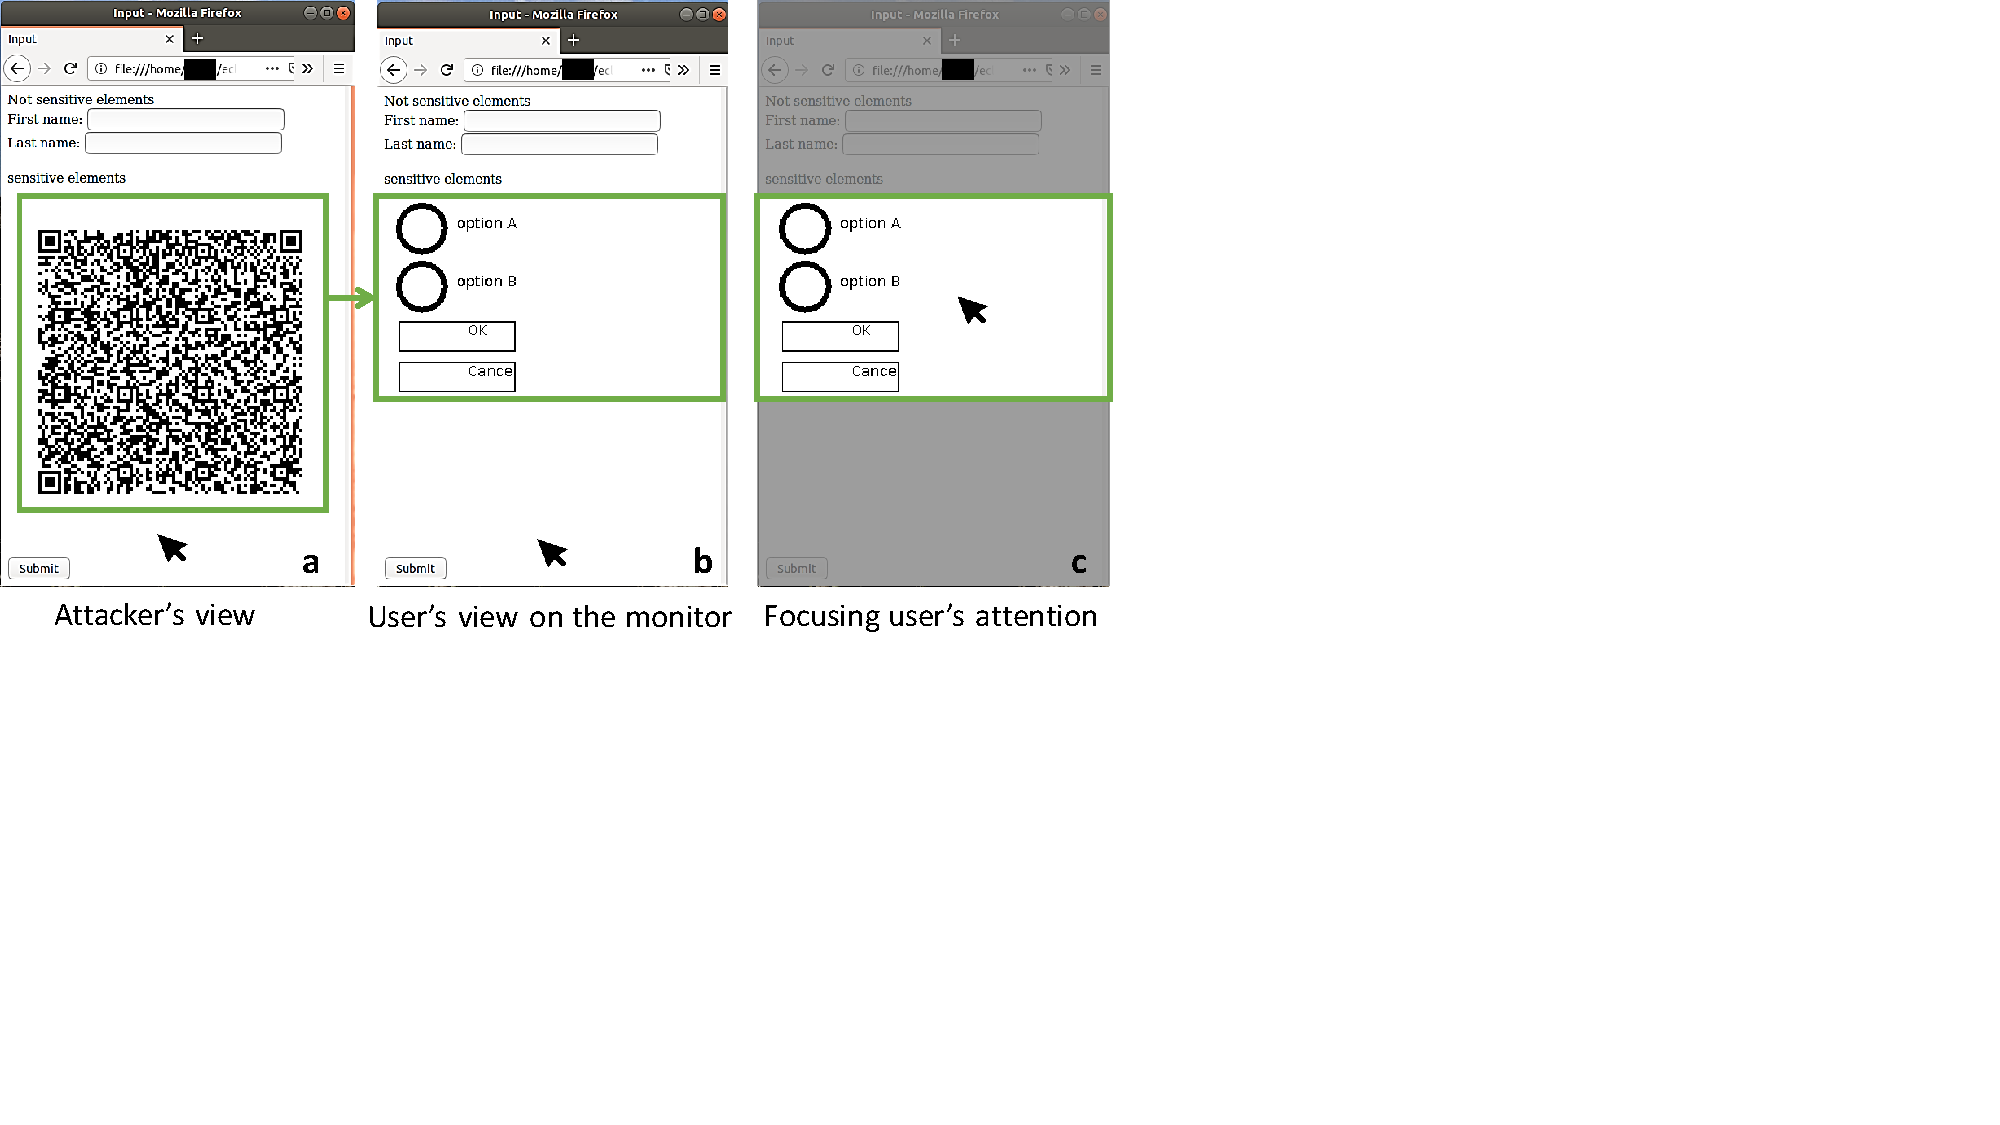
\includegraphics[trim={0 8cm 15cm 0}, clip, width=\linewidth]{chapters/ProtectIOn/images/overlayScreenShot_new.pdf}
\caption[\name's high-level approach for UI overlays]{\textbf{\name's high-level approach for UI overlays} shows that the \device generates UI overlay to protect IO integrity and confidentiality. a) The attacker only sees the non-protected UI elements, and the protected form is encrypted and encoded (in our case, the \device could decode a QR code and decrypt). b) shows the \device generated form overlay that is hidden from the host. The protected part of the screen provides integrity and confidentiality of all user IO. c) shows that the \device dims out (lightbox) the rest of the screen when the user moves her mouse pointer over the protected region to focus user attention.}

\label{fig:screenshot_1}
\end{figure}

\name is built upon the security requirements and functional properties that are described in Section~\ref{sec:problemStatement:goals}.
\device is active only when the user visits sensitive web applications that require \name security.
Initially, the remote server signs and delivers the sensitive UI elements to the host in a format that is understandable by \device. Next, the host transfers the sensitive UI to \device, and the \device verifies the signature to prevent manipulations by the host. As seen in a running example depicted in Figure~\ref{fig:screenshot_1}, the \device then renders the UI with sensitive elements into an overlay on top of the HDMI frame received from the host. Note that the host cannot access or modify the overlay generated by the \device. Also, the overlay covers only a part of the screen, allowing the other feature-rich content on the webpage to run unmodified. Therefore, this ensures that sensitive UI elements are presented to the user as expected by the remote server -- \emph{output integrity}. For the overlay, we use QR-codes to transfer data from the host to the device because we avoid using extra software/hardware for a separate channel, and it is easy to visualize.

When the user interacts (types or moves the pointer) with the overlay, \device does not forward any event from the keyboard or the mouse to the host. The interaction is maintained solely by \device, which renders on-screen user inputs and therefore offers a user experience that is identical to a typical one as if the \device is not present. The user clicks on the \emph{submit} button triggers the submission procedure, which consists of the \device signing the user inputs and sending it to the server. Note that the text fields of the form and the \emph{submit} button are inside the overlay, which is inaccessible by the host, hence the attacker cannot execute the early form submission or clickjacking attacks. Finally, the server verifies the signature of \device to guarantee that the host has not altered the data. Therefore, the \device ensures \emph{input integrity} for all \emph{modalities} of input.

For integrity guarantees, \name uses well-known user attention focusing mechanisms. Unlike systems like Fidelius, these mechanisms do not introduce any cognitive load to the users as \name does not rely on multiple security indicators. Mechanisms such as lightbox aid the user to distinguish the \device overlay on the screen from the rest. Thus, the untrusted host cannot trick the user into following malicious instructions when the user interacts with sensitive UI elements. In the case where confidentiality is required, the user manually triggers SAS, using a well-known sequences of keys such as \emph{Ctrl+Alt+Del} that highlights the sensitive UIs using mechanisms such as lightbox (see Section~\ref{sec:confidentiality:SAS} for details). For confidentiality, the host cannot observe the overlay and user input as they are encrypted by the TLS key between the \device and the server.

